\documentclass[a4paper,11pt]{report}
\usepackage[T1]{fontenc} % pour écrire en français
\usepackage[francais]{babel} %pour écrire en français
\frenchbsetup{StandardLists=true}
\usepackage[utf8x]{inputenc} %encodage en UTF-8
\usepackage{fancyhdr} %pour gérer les en-têtes et pieds de page
\usepackage{amsmath,amscd,amssymb} %pour insérer des expressions scientifiques
\usepackage[pdftex]{graphicx} %pour inclure des figures
\usepackage{subfig}
\usepackage{enumitem}
\usepackage{amssymb}
\usepackage{hyperref} %pour créer des liens hyper-textes
\usepackage{verbatim} %pour citer du code Latex ou autre
\usepackage{url} %pour citer une adresse web
\pagenumbering{arabic} %type de numérotation des pages
\graphicspath{{Figures/}} %les figures sont rangées dans le dossier Figures
\pagestyle{plain} %style des pages
%%%%%%%%%%%%%%%%%%%%%%%%%%%%%%%%%%%%%%%%%%%%%%%%%%%%%%%%%%%%%%%%%%%%%%%%%%%%%%%%%%%%%%%%%%%%%%%%%%
\begin{document}
%----------------------------------------------------------------------------------------------------------
% PAGE DE GARDE
%----------------------------------------------------------------------------------------------------------
\makeatletter
\def\clap#1{\hbox to 0pt{\hss #1\hss}}%
\def\ligne#1{%
\hbox to \hsize{%
\vbox{\centering #1}}}%
\def\haut#1#2#3{%
\hbox to \hsize{%
\rlap{\vtop{\raggedright #1}}%
\hss
\clap{\vtop{\centering #2}}%
\hss
\llap{\vtop{\raggedleft #3}}}}%
\def\bas#1#2#3{%
\hbox to \hsize{%
\rlap{\vbox{\raggedright #1}}%
\hss
\clap{\vbox{\centering #2}}%
\hss
\llap{\vbox{\raggedleft #3}}}}%
\def\maketitle{%
\thispagestyle{empty}\vbox to \vsize{%
\haut{}{\@blurb}{}
\vfill
\vspace{1cm}
\begin{flushleft}
\usefont{OT1}{ptm}{m}{n}
\huge \@title
\end{flushleft}
\par
\hrule height 4pt
\par
\begin{flushright}
\usefont{OT1}{phv}{m}{n}
\Large \@author
\par
\end{flushright}
\vspace{3.5cm}
\centering

\includegraphics[width=0.4\textwidth]{Photo_univlemans}
\hfill
\vfill
\bas{}{\@location}{}
}%
\cleardoublepage
}
\def\author#1{\def\@author{#1}}
\def\title#1{\def\@title{#1}}
\def\location#1{\def\@location{#1}}
\def\blurb#1{\def\@blurb{#1}}
\author{}
\title{}
\location{Le Mans}\blurb{}
\makeatother
\title{\textbf{SPAM}: \textbf{S}ynchronisation de \textbf{P}endules \textbf{A}ppliquée aux \textbf{M}\'etronomes}
\author{Tony Merrien \& R\'emi Plantade}
\location{Le Mans, Année Universitaire 2014-2015}
\blurb{%
Université du Maine\\
Faculté des Sciences
\textbf{Rapport de projet}\\[1em]
Semestre 3 L2 SPI\\
Encadrant : Mr. Guillaume Penelet, Enseignant-chercheur
}
%%%%%%%%%%%%%%%%%%%%%%%%%%%%%%%%%%%%%%%%%%%%%%%%%%%%%%%%%%%%%%%%%%%%%%%%%%%%%%%%%%%%%%%%%%%%%%%%%%
\maketitle %génère la page de garde
\newpage
\pagenumbering{roman} \setcounter{page}{1} %les pages commencent à être numérotées en lettre romaines.
%%%%%%%%%%%%%%%%%%%%%%%%%%%%%%%%%%%%%%%%%%%%%%%%%%%%%%%%%%%%%%%%%%%%%%%%%%%%%%%%%%%%%%%%%%%%%%%%%%
\newpage
\null
\thispagestyle{empty}
\newpage
%------------------------------------------------------------------------------------------------------
% TABLE DES MATIÈRES
%------------------------------------------------------------------------------------------------------
{\tableofcontents}
%\newpage\
\listoffigures
\newpage
%%%%%%%%%%%%%%%%%%%%%%%%%%%%%%%%%%%%%%%%%%%%%%%%%%%%%%%%%%%%%%%%%%%%%%%%%%%%%%%%%%%%%%%%%%%%%%%%%%%%%%%%%%%%%%%%
\chapter*{Introduction}
\addcontentsline{toc}{chapter}{Introduction} %Ce chapitre n'est pas numéroté mais apparaitra dans la table des matières gràce à cette commande.
\pagenumbering{arabic} \setcounter{page}{1} %Le numéro de page est remis à zéro et la numérotation est en chiffre arabe
	La synchronisation est un phénomène universellement observable et étudié depuis des siècles. Une foule qui applaudit, le chant de criquets, les piles cardiaques et les métronomes étudiés dans l'ensemble de ce projet sont les conséquences, enjeux et applications directement observables de ce phénomène physique.\\

	La synchronisation est le terme utilisé, dans un sens large, pour caractériser une coordination d'opérations au cours du temps. Découvert en 1665 par Christiaan Huygens alors qu'il cherchait à aider les hommes partant en mer pour de longues périodes afin de déterminer la longitude, chose difficile si la mesure du temps est peu précise. Il constata que deux pendules solidaires d'un support finnissaient toujours par se synchroniser avec une certaine phase.\\

	Dans le prolongement d'une étude précédement effectuée par deux étudiants en L3 SPI, ce projet dans son aspect de recherche mettera en corrélation, dans un premier temps, les observartions déja éffectuées et, par la suite, approfondira les aspects expérimentaux. Le phénomène est étudié en détails à l'aide de différentes manipulations mettant en oeuvre toujours deux métronomes mécaniques. Ces expériences sont éffectuées sur un banc de mesure explicité plus loin. Les résultats obtenus sont interpretés et traités numériquement pour mettre en relation théorie et experiences.

\newpage
\null
\thispagestyle{empty}
%%%%%%%%%%%%%%%%%%%%%%%%%%%%%%%%%%%%%%%%%%%%%%%%%%%%%%%%%%%%%%%%%%%%%%%%%%%%%%%%%%%%%%%%%%%%%%%%%%
\chapter{La synchronisation}
%%%%%%%%%%%%%%%%%%%%%%%%%%%%%%%%%%%%%%%%%%%%%%%%%%%%%%%%%%%%%%%%%%%%%%%%%%%%%%%%%%%%%%%%%%%%%%%%%%
\section{Définitions}
Dans cette partie, l'intégralité du projet, des hypothèses, du matériel, des phénomènes, des définitions et du procédé expérimental est développé.\\
\underline{Synchronisation (universelle)}: "Coordination de plusieurs opérations entre elles en fonction du temps"\cite{wiki}\\
\underline{Synchronisation (scientifique)}: "Procédé pour rendre synchrones deux systèmes oscillant mécaniquement de manière indépendante"\cite{cntrl}\\
\underline{Pendule}: "Corps ou système matériel capable d'osciller en un point fixe"\cite{ikonet}\\
\underline{Métronome}: "Appareil pendulaire mû par un ressort dont on peut régler la pulsation."\cite{pend} \\

\section{Matériel}

La liste du méteriel utilisé est la suivante:\\
\begin{itemize}[label=\textbullet, leftmargin=* ,parsep=0cm,itemsep=0cm,topsep=0cm]
\item Carte d'acquisition National Instruments ;
\item Deux microphones Roga Instruments MI-17 ;
\item Deux pieds microphoniques ;
\item Deux canettes ;
\item Un pot vibrant ;
\item Préamplificateur BSWA MC102 ;
\item Bloc de mousse
\item Deux métronomes mécaniques ;
\item Un support rectangulaire plat ;
\item Logiciel CTTM ;
\item Logiciel Matlab
\end{itemize}

\section{Banc de mesure}

Le matériel est utilisé de la manière suivante: la plaque (ici en bois) est placée sur deux canettes parallèles entre elles, la même où sont placés les deux métronomes mécaniques. Deux microphones, reliés à la carte d'acquisition par le biais d'un préamplificateur, sont placés proches de chaque métronomes afin de relever les clics sonores de ceux-ci, séparés par un bloc de mousse acoustiquement isolante.\\
\begin{figure}[h]
\centering
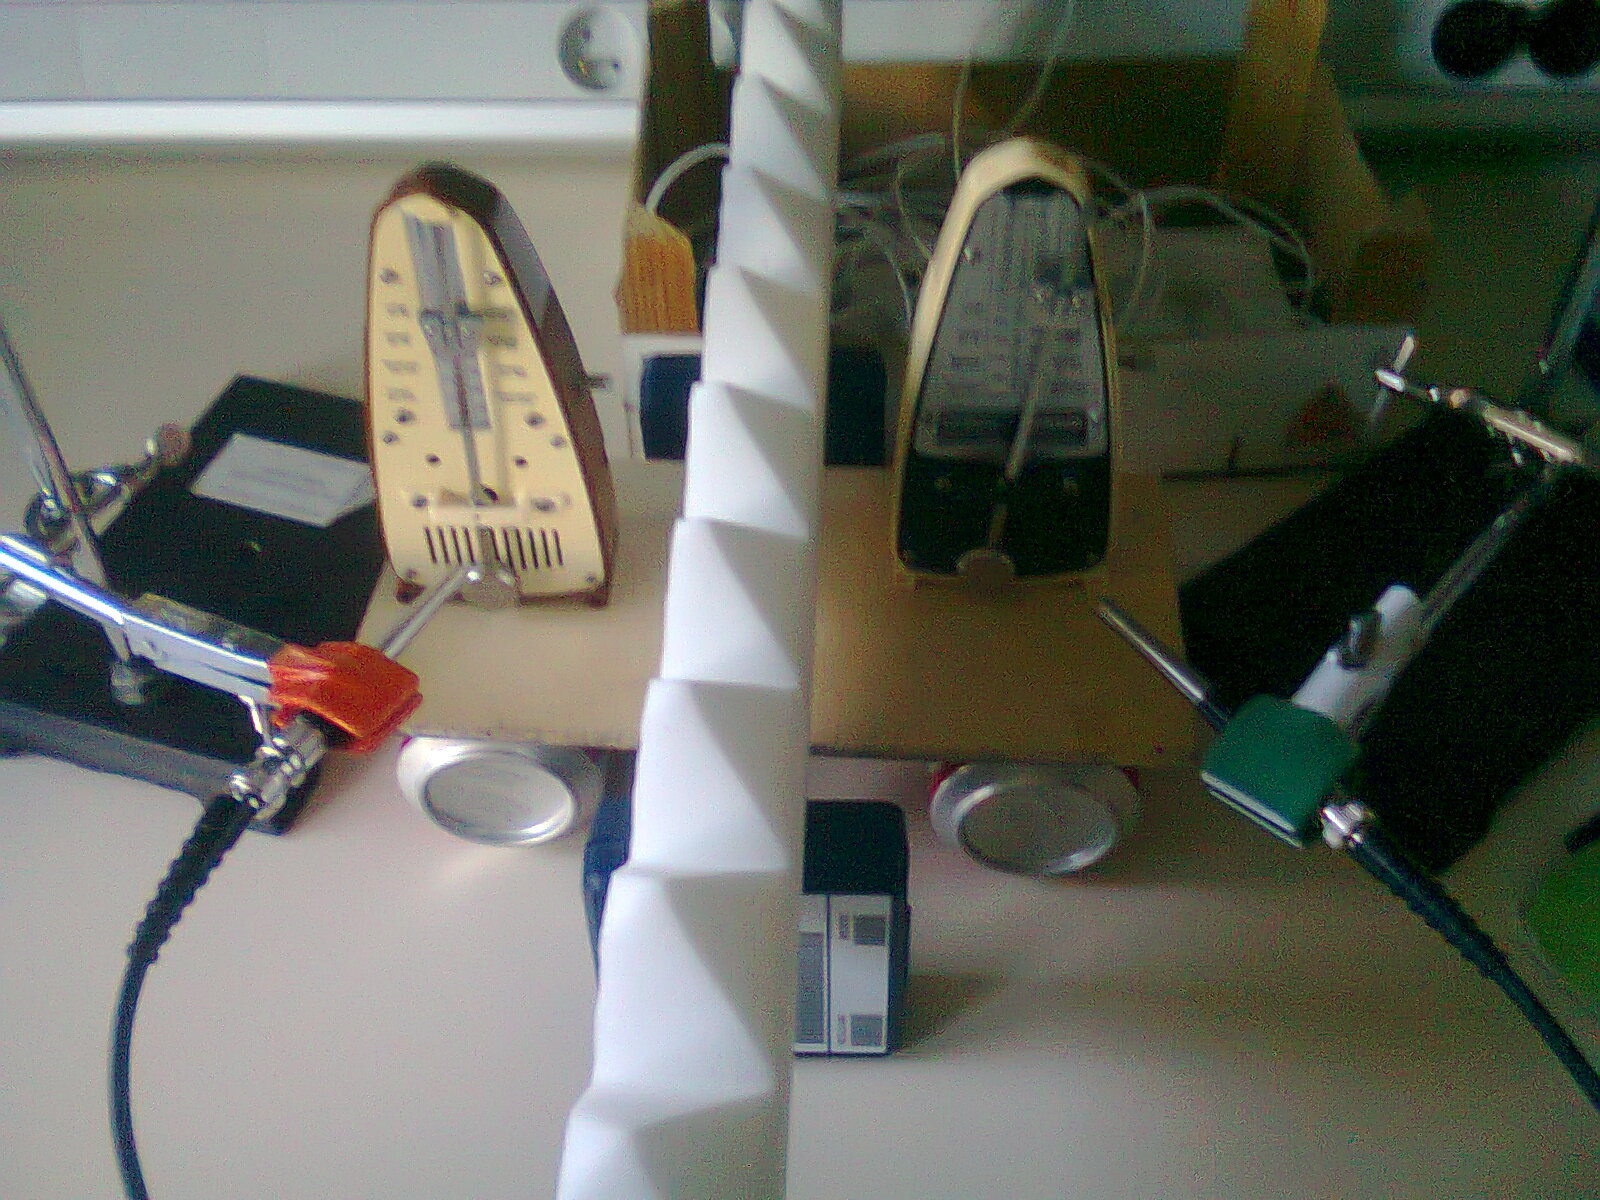
\includegraphics[width=0.6\textwidth]{BancMesure}
\caption{Banc de mesure}\label{Banc}
\end{figure}\\
Ce dispositif permet d'isoler de manière sonore chaque clic des métronomes et ainsi faciliter un traitement numérique ultérieur, sans inteférer sur le système d'une quelconque manière.
%%%%%%%%%%%%%%%%%%%%%%%%%%%%%%%%%%%%%%%%%%%%%%%%%%%%%%%%%%%%%%%%%%%%%%%%%%%%%%%%%%%%%%%%%%%%%%%%%%
\chapter{Experiences}
%%%%%%%%%%%%%%%%%%%%%%%%%%%%%%%%%%%%%%%%%%%%%%%%%%%%%%%%%%%%%%%%%%%%%%%%%%%%%%%%%%%%%%%%%%%%%%%%%%
\section{Fonctionnement d'un métronome}
La réalisation des expériences étant maintenant permise, il est nécessaire de caractériser  l'ensemble de l'équipement. Par suite de ce rapport, on prend un soin particulier à faire la différence entre battement d'un métronome (BPM) et fréquence d'oscilation (Hz). Dans une approche de meilleure compréhension d'un auto oscillateur mécanique, un métronome est  démentelé. Il est bénéfique d'avoir une meilleure compréhension de leurs mécanismes internes. Ainsi il est remarqué que remonter un métronome est en fait l'action qui tend le ressort interne servant de mécanisme d'action sur le balancement de la masse. Il est donc nécéssaire de remonter régulièrement, pour des précisions optimales, les métronomes. \\

\section{Caractérisation de l'équipement}
Avant toute manipulation, afin de simplifier les explications, on utilisera le terme "{\it Mr White}" pour désigner le métronome blanc et "{\it Mr Brown}" pour désigner le métronome marron. Suite à divers experiences, les valeurs de battements inscrites sur lesappareils sont peu fiables. Celles indiquées ne sont pas les véritables battements des métronomes. De ce fait, ceux-ci sont caractérisés de manière précise pour chaque mesure de synchronisation. Le programme présenté en \underline{Annexe \ref{Battements}}, est crée pour calculer le véritable battement des métronomes en fonction du temps. Ainsi, pour chacune des mesures suivantes, ce n'est pas la valeur présentée sur métronome qui sera prise en compte, mais celle obtenue par le l'analyse numérque éffectuée de manière systématique.

\section{Synchronisation Experimentale}

\subsection{Synchronisation pour différents battements}
	A présent l'étude dans cette partie se porte sur la synchronisation pour une différence de fréquence entre les deux métronomes. Sachant que le phénomène commence à se produire pour au moins 176 BPM, Mr.Brown est réglé sur 180 BPM tandis que Mr.White sur un battement par minute plus faible afin de trouver la limite inférieur où il y a synchronisation. Les deux métronomes sont disposés sur le système afin de déterminer si il y a ou non synchronisation. Si le phénomène se produit alors les deux métronomes sont posés sur la table et leur fréquence est mesurés et traité par un programme. On réitère cette manipulation jusqu'à tomber sur la limite de la différence de fréquence entre les deux métronomes pour qu'il y est synchronisation.   Ensuite Mr.Brown reste fixé a 176 BPM et Mr.White est réglé pour une fréquence supérieure pour que de même que précédemment déterminer la limite mais cette fois si la limite supérieur de la synchronisation pour une différence de fréquences entre les deux métronomes. Cette procédure est répétée pour trouver, suivant la fréquence fixe, les limites et ainsi tracer une courbe afin d'en tiré une analyse du comportement.( a revoir la formulation). 
	
					TITRE !!!
					
					COURBE !!!
					
					LEGENDE !!!
					
					EXPLICATION DE LA COURBE OBTENUE !!!
					
Une étude est ensuite menée afin de savoir si il y a une synchronisation possible pour des fréquences harmoniques, c'est à dire un métronome fixé à une certaine fréquence f0 et l'autre métronome à un fréquence 2 fois plus ou moins élevé. La manipulation est réalisée avec Mr.Brown réglé à 208BPM et Mr.White à 104BPM. L'expérience n'est pas concluante. En effet précédemment un seuil de fréquence pour obtenir une synchronisation a été trouvé, 176 BPM , or ici Mr.White est réglé à 104BPM qui est bien inférieur au seuil. Les métronomes pouvant allés que jusqu'à 230BPM l'étude sur la synchronisation en régime harmonique est compromise. 

\subsection{Synchronisation par harmonique}

\section{Limite de synchronisation}
La synchronisation opère dans une bande fréquence bien définie. Pour une fréquence imposé à un métronome, la synchronisation opère de manière différentes pour des battements différents. Après avoir étudié et caractérisé le matériel mise à notre disposition, l'étude du phénomène est entamé avec différentes expériences. La synchronisation de métronomes ayant été déjà traité, les premières expériences ont pour but de vérifier les informations obtenues dans le précédent rapport. Lors de la première expérience avec notre banc de mesure, la limite de fréquence des deux métronomes pour qu'il y est synchronisation est recherchée. Pour cela les deux métronomes sont réglés, par le biais de la position de la masselotte sur la tige pour obtenir un battement par minute (BPM) faible, ce qui signifie que la fréquence est basse, environ 50 BPM pour les deux lors de cette première manipulation. Le phénomène ne se produisant pas les métronomes sont réglés sur une autre fréquence plus élevée et la manipulation est renouvelée. Ainsi avec cette expérience la détermination d'une limite de fréquence pour l'observation du phénomène de synchronisation est obtenue. Les résultats acquis sont en accord avec ceux du rapport des L3 \cite{ram}. En effet la synchronisation entre deux métronomes ne s'effectue pas en basse fréquence et un seuil a été déterminé, qui se situe à 176 BPM. La limite de déplacement de la massette sur le métronome empêche la détermination d'un éventuel seuil de haute fréquence où le phénomène ne se produit plus. Au cours de l'expérience, lorsque les deux métronomes se synchronisent ils sont en opposition de phase. En effet lorsque les métronomes sont désynchronisés la plaque se déplace sur les cannettes tandis que lorsque les deux métronomes sont synchronisés en opposition de phase la plaque reste immobile, le système est donc à son état d'équilibre. Le transfert d'énergie le plus faible possible entre les deux métronomes et le système (plaque en bois et les deux cannettes) est donc naturellement privilégié.

\section{Pot Vibrant}
Dans cette partie l'étude se porte sur la synchronisation des deux métronomes avec un pot vibrant relié à la plaque en bois. Le pot vibrant est un objet permettant d'exciter le système par le biais, ici, d'un pas de vis relié avec une vis à la plaque en bois. La fréquence d'excitation et son amplitude sont réglés avec l'amplificateur relié au pot vibrant. Le dispositif experimental est le suivant:
\begin{figure}[h]
\centering
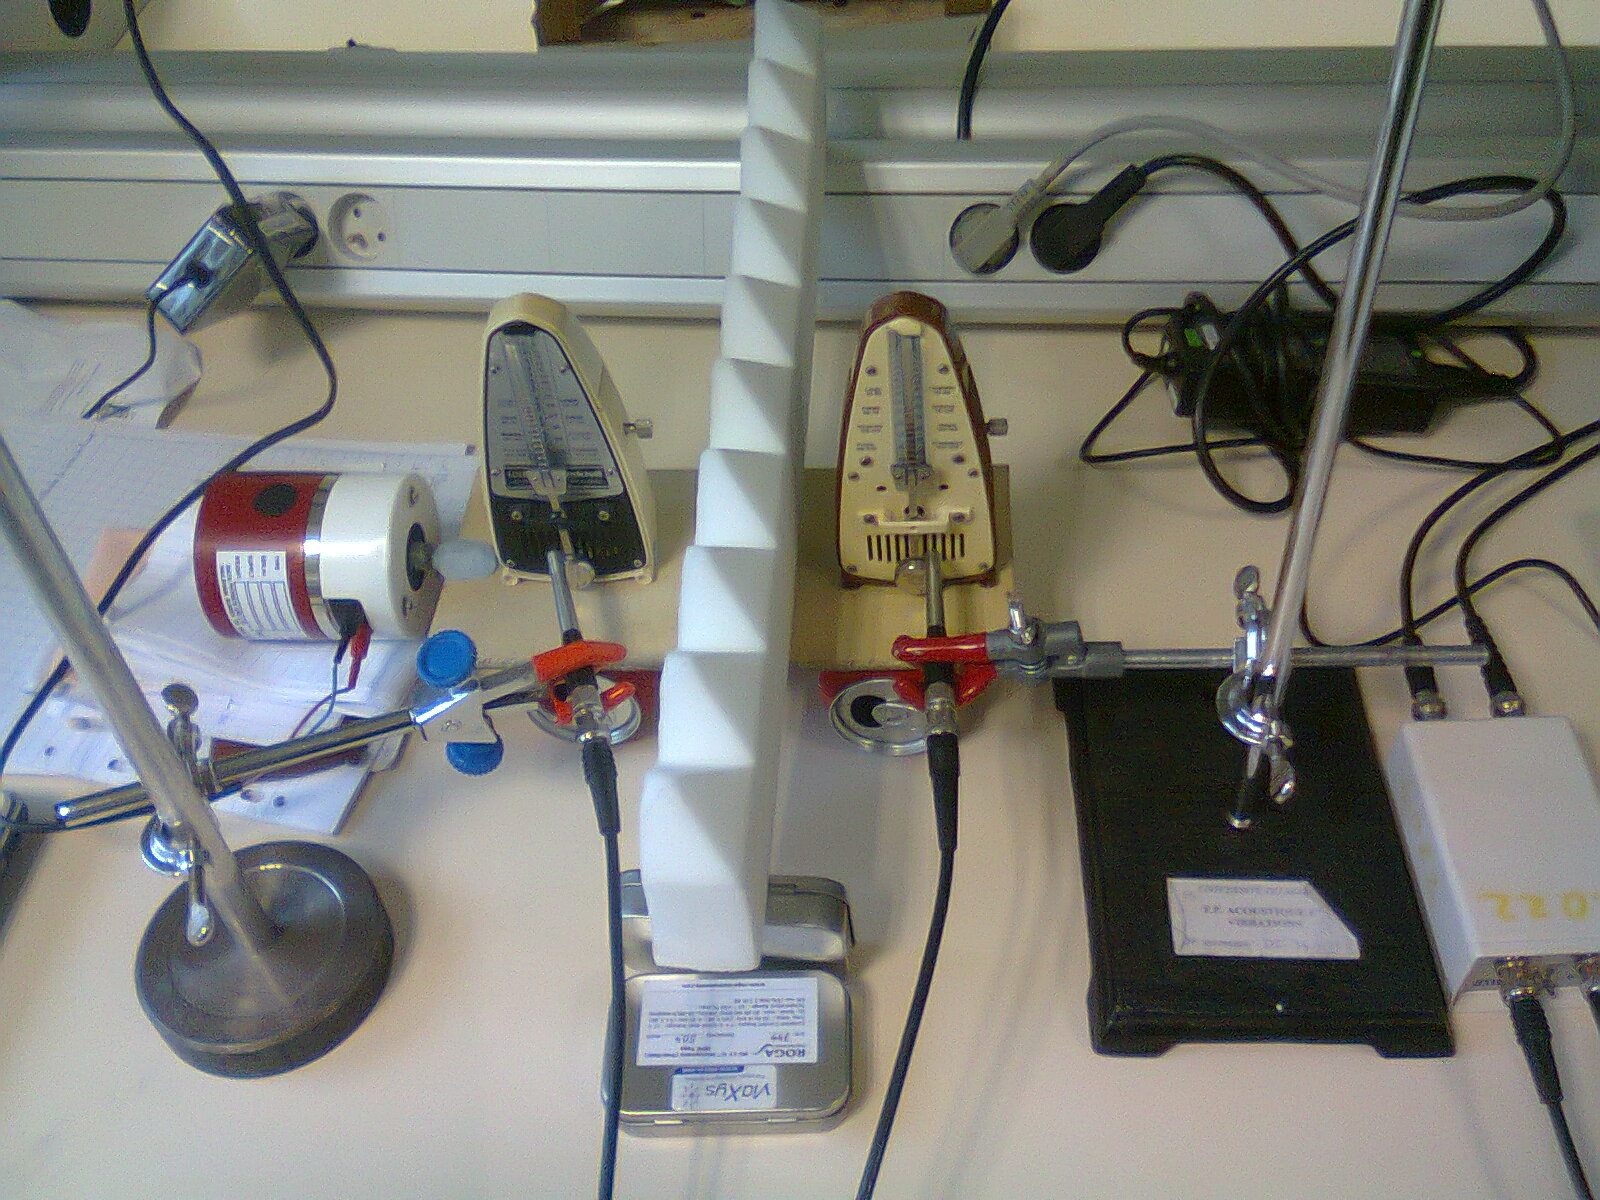
\includegraphics[width=0.6\textwidth]{Bancpotvibrant}
\caption{Banc de mesure avec un pot vibrant}\label{BancPot}
\end{figure}\\

FORMULE POUR PASSER DES BPM AU HERTZ

L'expérience réalisée ici consiste à donner à la plaque en bois une certaine fréquence d'excitation correspond à la fréquence d'oscillation du métronome suivant où est placé la masselotte et une amplitude d'oscillation au système(à reformuler).
Ainsi avec ce nouveau banc de mesure il est possible d'étudier si les limites de la synchronisation change et d'observer l'influence de l'amplitude sur la synchronisation.
 

%%%%%%%%%%%%%%%%%%%%%%%%%%%%%%%%%%%%%%%%%%%%%%%%%%%%%%%%%%%%%%%%%%%%%%%%%%%%%%%%%%%%%%%%%%%%%%%%%%
\chapter{Analyse Numérique}
%%%%%%%%%%%%%%%%%%%%%%%%%%%%%%%%%%%%%%%%%%%%%%%%%%%%%%%%%%%%%%%%%%%%%%%%%%%%%%%%%%%%%%%%%%%%%%%%%%
\section{Comparaison théorie}
Le traitement des données enregistrés est effectué dans cette partie par le biais d'un programme de traitement présenté en \underline{Annexe \ref{Traitement}}, basé sur le rapport des L3\cite{ram}. Les courbes obtenues sont analysées et comparées avec le modèle théorique. Précisons que la théorie ici n'est pas mathématique, mais est celle énoncé de manière écrite dans les différentes ouvrages bibliographiques contribuant à l'élaboration de ce rapport.
\subsection{Interprétation de la caractérisation}
Dans un premier temps, lors de la caractérisation de chaque métronome dans un cas général, les courbes suivantes sont obtenues. En premier lieu, l'évolution temporelle des clics des métronomes est la suivante:
\begin{figure}[h]
\centering
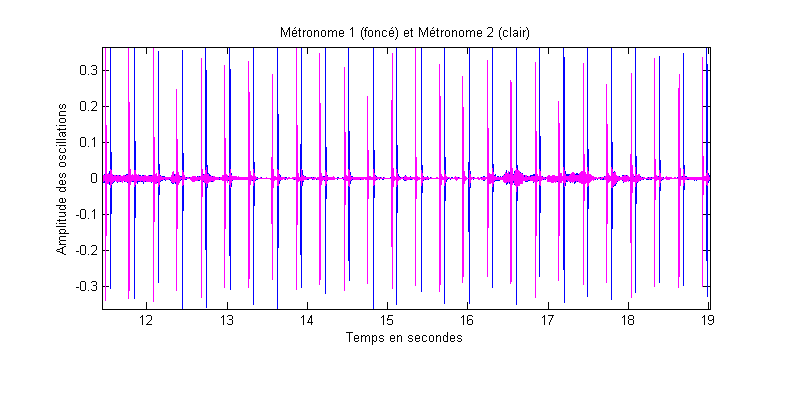
\includegraphics[width=1\textwidth]{Caracterisation_temporelle_200BPM}
\caption{Evolution temporelle de deux métronomes déssolidarisés aux fréquences différentes}\label{CaractérisationT}
\end{figure}\\

On remarque distinctement deux battements périodique dans le temps. Ensuite il est possible de voir leurs évolutions fréquentielles :
\begin{figure}[h]
\centering
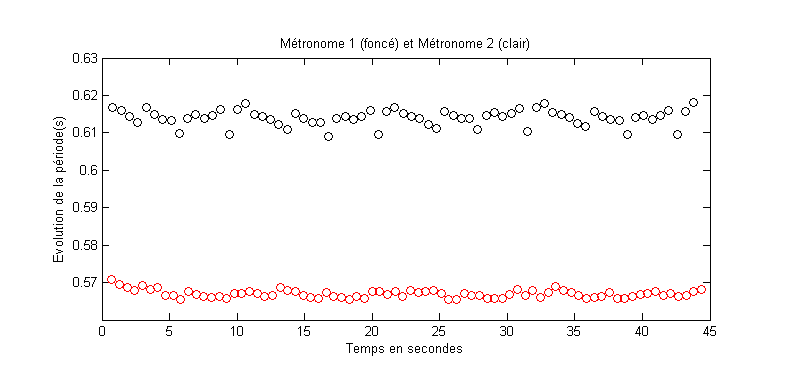
\includegraphics[width=1\textwidth]{Caracterisation_Frequence_200BPM}
\caption{Evolution fréquentielle de deux métronomes déssolidarisés au cours du temps}\label{CaractérisationF}
\end{figure}\\

Les deux métronomes sont bien à des fréquences différentes. On pet aussi voir qu'un métronome mécanqiue bat difficilementde manière constante fréquentiellement.
Enfin, puisque les fréquences d'oscillations sont connues, on peut afficher graphiquement la différence de périodes, synonymes lorsque celle ci tend vers 0, de la présence de synchronisation car varation de période d'oscillation :
\begin{figure}[h]
\centering
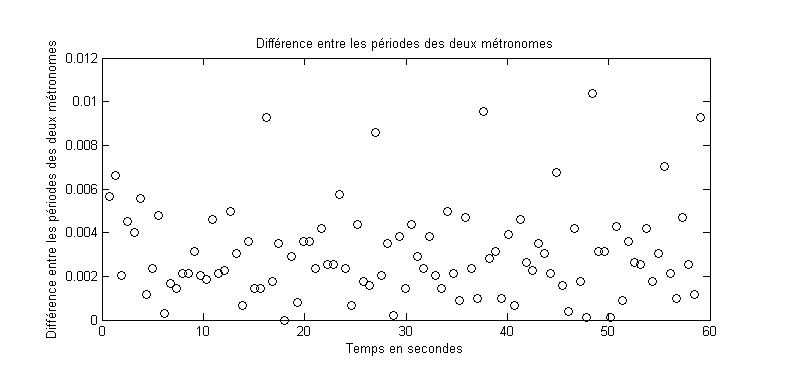
\includegraphics[width=1\textwidth]{Caracterisation_Periode_200BPM}
\caption{Evolution de la différence de période de deux métronomes déssolidarisés au cours du temps}\label{CaractérisationP}
\end{figure}\\
On peut donc obsever l'abscence totale de synchronisation.
\subsection{Interprétation de la synchronisation}
Dans cette partie, les analyses précédentes sont répétées dans le cas où les métronomes sont solidaires du support posé sur deux canettes. Ainsi l'évolution temporelle des clics :
\begin{figure}[h]
\centering
\includegraphics[width=1\textwidth]{Synchro_Temporelle_208BPM}
\caption{Evolution temporelle de deux métronomes solidaire d'un support au cours du temps}\label{SynchronisationT}
\end{figure}\\
Ici, une synchronisation apparait dans les 10 premières secondes de la mesure éffectuées.
L'évolution fréquentielle et de la différence de période sont les suivantes:
\begin{figure}[h]
\centering
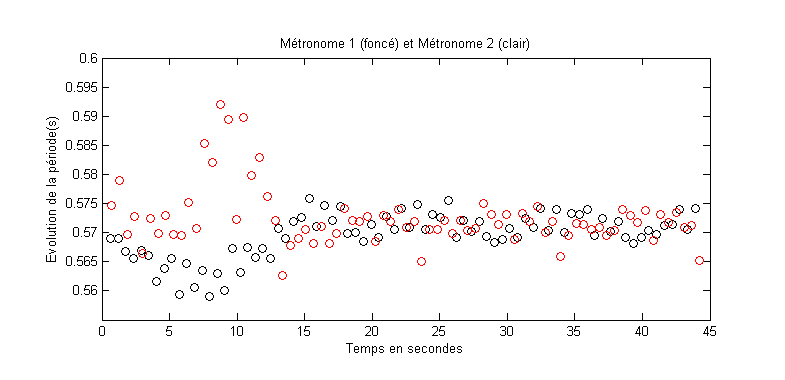
\includegraphics[width=1\textwidth]{Synchro_Frequence_208BPM}
\caption{Evolution fréquentielle des deux métronomes solidaire d'un support au cours du temps}\label{Synchronisation}
\end{figure}\\
Il est dans ce cas très aisé d'obsver une synchronisation.

Harnold Tongues + courbe théorique

\section{Pot vibrant}

amplitude courbe

\section{"Trap phase"}

bla bla bla
%%%%%%%%%%%%%%%%%%%%%%%%%%%%%%%%%%%%%%%%%%%%%%%%%%%%%%%%%%%%%%%%%%%%%%%%%%%%%%%%%%%%%%%%%%%%%%%%%%
\chapter*{Conclusion}
%%%%%%%%%%%%%%%%%%%%%%%%%%%%%%%%%%%%%%%%%%%%%%%%%%%%%%%%%%%%%%%%%%%%%%%%%%%%%%%%%%%%%%%%%%%%%%%%%%
\addcontentsline{toc}{chapter}{Conclusion} %permet d'inclure le chapitre conclusion dans la table des matières
La synchronisation est un phénomène assez simple a observer et analyser qui peut s'avérer complexe dans son intérprétation et le champs de possiblilité d'exploration qu'il offre. Il est donc très enrichissant de s'impliquer dans une démarche d'analyse et de compréhension.
%%%%%%%%%%%%%%%%%%%%%%%%%%%%%%%%%%%%%%%%%%%%%%%%%%%%%%%%%%%%%%%%%%%%%%%%%%%%%%%%%%%%%%%%%%%%%%%%%%
%bibliography
\renewcommand{\bibname}{Références}
\begin{thebibliography}{2}
\section*{Bibliographie}
% \bibitem[label]{cle} Auteur, TITRE, editeur, annee
\bibitem{piko} A. PIKOVSKY, {\it Synchronisation, A universal concept in nonlinear sciences, Cambridge Nonlinear Science Series 12, 2001}
\bibitem{panta} J. PANTALEONE, {\it Synchronization of metronomes, Am. J. Phys., Vol. 70, No 10, October 2002}
\bibitem{ram} M. RAMSEIER, M. ROBIN, {\it Projet L3 SPI: hénomène de Synchronisation de Pendules Appliqué aux Métronomes, 2012}
\section*{Webographie}
\bibitem{wiki} \url{http://fr.wikipedia.org/wiki/Synchronisation}
\bibitem{cntrl} \url{http://www.cntrl.fr/lexicographie/synchronisation}
\bibitem{ikonet} \url{http://ikonet.com/fr/ledictionnairevisuel/arts-et-architecture/musique/accessoire/metronome-mecanique.php}
\bibitem{pend} \url{http://www.cntrl.fr/lexicographie/pendule}
\end{thebibliography}
%%%%%%%%%%%%%%%%%%%%%%%%%%%%%%%%%%%%%%%%%%%%%%%%%%%%%%%%%%%%%%%%%%%%%%%%%%%%%%%%%%%%%%%%%%%%%%%%%%
\appendix
\chapter{Analyse numérique: Calcul du battement d'un métronome}
\label{Battements}
\begin{verbatim}
%Programme pour déterminer le nombre de transitoire(s) (donc la fréquence
%d'oscillation) d'un métronome :
clear all
close all
%On charge le fichier à analyser (celui-ci dois durer 45 secondes)
D = load('Synchro Pot Vibrant 200 BPM.txt');
%On défini la taille du tableau contenu dans le fichier
taille = length(D(:,1));
%On déclare deux variables qui contiendront le nombre de transitoire de
%chaque métronome
n1=0;
n2=0;
%On crée une valeur temporaire d'incrémentation
i = 1;

while(i<taille)
    abs(D(i,1));
    if(abs(D(i,2)) > 0.25)
        n1 = n1+1;
        i = i+500;
    end
    i = i+1;
end
%On affiche maintenant n1
n1 = (n1*60/45)
i = 1;

while(i<taille)
    abs(D(i,1));
    if(abs(D(i,3)) > 0.25)
        n2 = n2+1;
        i = i+500;
    end
    i = i+1;
end
%On affiche maintenant n2
n2 = (n2*60/45)
\end{verbatim}
%%%%%%%%%%%%%%%%%%%%%%%%%%%%%%%%%%%%%%%%%%%%%%%%%
\chapter{Analyse numérique: Traitement des données}
\label{Traitement}
\begin{verbatim}
%Programme traçant l'évolution de la période de
%chacun des métronomes au cours du temps :
clear all;
close all;
%On charge dans un premier temps le fichier texte contenant
%les mesures prises expérimentalement dans la matrice 'D' :
D = load('Synchro Max.txt');
%On place la première colonne de la matrice 'D'
%(correspondant aux données temporelles) dans le vecteur 't' :
t=D(:,1);
%La variable 'Te' est créée. Elle a pour valeur
%celle de la deuxième case du vecteur 't'.
%Elle correspond ‡ la période d'échantillonnage :
Te = t(2);
%La deuxième colonne de la matrice 'D' est placée dans le vecteur 'm1'.
%Celle-ci correspond aux donnÈes enregistrées pour le premier métronome :
m1 = abs(D(:,2));
%La troisième colonne de la matrice 'D' est placée dans le vecteur 'm2'.
%Celle-ci correspond aux donnÈes enregistrÈes pour le deuxième métronome :
m2 = abs(D(:,3));
%On cherche l'amplitude maximale dans chaque vecteur 'm1' et 'm2' et
%on les appelle respectivement 'M1' et 'M2' :
M1 = max(m1);
M2 = max(m2);
%'C' est le rapport de 'M1' et de 'M2' :
C = M1/M2;
%On divise chaque maximum par une valeur choisie arbitrairement afin de
%définir un seuil. Ce seuil servira à identifier les 'tac' du métronome :
M1 = M1/3;
M2 = M2/2;
%'L' correspond au nombre de point contenu dans 'm1'
%(qui est le mÍme que celui dans 't' et dans 'm2') :
L = length(m1);
%On initialise les compteurs 'n1' et 'n2' :
n1=0;
n2=0;
%On initialise la variable 'durée' (choisie arbitrairement)
%qui détermine un pas minimum entre deux 'tac' :
duree = 20e-2;
%On initialise les variables 'T1' et 'T2' qui controlent que le pas
%appelé 'duree' est bien respecté :
T1 = 0;
T2 = 0;
%On créé une boucle qui sert à compter le nombre de 'tac'
%effectué par chaque mÈtronome au court de l'expérience :
for i = 1 : 1 : L
%Pour ce faire, on regarde si l'amplitude du point numéro 'i'
%du vecteur 'm1' et 'm2' est supÈrieur au seuil 'M1 et 'M2' :
if m1(i) > M1
%On regarde si la coordonÈe temporelle du 'tac' en i est bien espacée
%au minimum du pas 'duree' par rapport à l'ancien 'tac' :
if t(i) - T1 > duree
%Si c'est le cas, on incrémente le compteur correspondant
%au vecteur de 1 ('n1' pour 'm1' et 'n2' pour 'm2') :
n1 = n1+1;
%On change la valeur de 'T1' par la coordonée temporelle du premier pic :
T1 = t(i);
end
end
if m2(i) > M2
if t(i) - T2 > duree
n2 = n2+1;
T2 = t(i);
end
end
end
%On divise ensuite chaque compteur par deux. En effet,
%les battements du métronome sont espacés d'une demi-période :
%Le nombre de période d'oscillation effectuées par chaque métronome
%est donc Ègal ‡ la moitié de 'n1' et 'n2' :
n1 = n1 / 2;
n2 = n2 / 2;
%On ne prend que la partie entière de chacun des compteurs
%afin d'éviter le cas où le nombre de demi-période est impaire :
n1 = floor(n1);
n2 = floor(n2);
%On initialise les variables 'z1' et 'z2' ‡ 0 :
z1 = 0;
z2 = 0;
%On créé les vecteurs 'V1' et 'V2' contenant
%respectivement 'n1' et 'n2' lignes de 0 :
V1 = zeros(n1,1);
V2 = zeros(n2,1);
%On initialise les compteurs k1 et k2 :
k1 = 1;
k2 = 1;
%On réinitialise les variables T1 et T2 ‡ 0 :
T1 = 0;
T2 = 0;
%On créé une boucle qui permet de compter le nombre de période
%effectuée par chaque mÈtronome au cours de l'expérience :
for i = 1:1:L
%Pour ce faire, on regarde si chaque valeur des vecteurs
%'m1' et 'm2' est supérieure aux seuils 'M1' et 'M2' :
if m1(i) > M1
%On regarde si la coordonnÈe temporelle de l'ancien pic et celle
%du nouveau pic sont bien expacées de 'duree' secondes :
if t(i) - T1 > duree
%Si c'est le cas, on remplace la variable T1 par la valeur de t(i) :
T1 = t(i);
%Les variables 'z1' et 'z2' servent ‡ prendre un battement sur deux
%afin d'obtenir des période et non des demi-périodes :
if z1 == 0
%En effet, si 'm1(i)>M1', on regarde si 'z1==0'. Si c'est le cas on prend
%la coordonnée temporelle 't(i)' correspondant ‡ 'm(i)' et on la place dans
%'V(k1)'. Puis on incrémente 'k1' et on remplace 'z1' par la valeur 1 :
V1(k1) = t(i);
k1 = k1+1;
z1 = 1;
%On vérifie que 'k1' n'est pas supérieur ‡ 'n1' afin de ne pas dépasser
%la taille du vecteur. Si c'est le cas, on stop la boucle :
if k1 > n1
break;
end
%Si 'z1==1', on change la valeur de 'z1' et on
%recommence la boucle pour 'i=i+1' :
elseif z1 == 1
z1=0;
end
end
end
end
%On effectue la même chose pour le deuxième métronome :
for i = 1 : 1 : L
if m2(i) > M2
if t(i) - T2 > duree
T2 = t(i);
if z2 == 0
V2(k2) = t(i);
k2 = k2+1;
z2 = 1;
if k2 > n2
break;
end
elseif z2 == 1
z2=0;
end
end
end
end
%On créé les vecteurs 't1' et 't2' contenant
%chacun 'n1-1' et 'n2-1' lignes de 0 :
t1 = zeros(n1-1,1);
t2 = zeros(n1-1,1);
%On créé les vecteurs 'P1' et 'P2' contenant
%chacun 'n1-1' et 'n2-1' lignes de 0 :
P1 = zeros(n1-1,1);
P2 = zeros(n2-1,1);
%On créé une boucle remplaÁant chaque valeur de 'P1' et 'P2' par
%la diffÈrence entre la coordonnée temporelle de chaque période.
%Par exemple, si l'on dÈbute la premiËre pÈriode ‡ 5s et la deuxième
%‡ 5,1s, V(i)=5 et V(i+1) = 5,1, et donc P1(k1) = 0,1s qui est la valeur
%de la première période.On remplace la valeur i du vecteur t1 par la moyenne
%des valeurs i et i+1 du vecteur V. On obtient ainsi la localisation temporelle
%de la pÈ-ériode :
for i = 1 : 1 : n1-1
P1(i) = V1(i+1)-V1(i);
t1(i) = (V1(i+1)+V1(i))/2;
end
%On fait de mÍme avec le métronome 2 :
for i = 1 : 1 : n2-1
P2(i) = V2(i+1)-V2(i);
t2(i) = (V2(i+1)+V2(i))/2;
end
%On multiplie les valeurs des amplitudes du mÈtronomes 2 par
%'C' afin d'avoir des amplitudes comparables pour les deux signaux :
D(:,3) = D(:,3)*C;
%La figure 1 trace en haut l'évolution de la période de chacun des
%métronomes et en bas les signaux temporels de chacun des métronomes :
figure (1)
subplot(2,1,1)
plot(t1,P1,'go')
hold on
plot(t2,P2,'ro')
xlabel('Temps en secondes')
ylabel('Evolution de la période(s)')
title('Métronome 1 (vert) et Métronome 2 (rouge)')
subplot(2,1,2)
plot(t,D(:,2),'m')
hold on
plot(t,D(:,3),'c')
xlabel('Temps en secondes')
ylabel('Amplitude des oscillations')
title('Métronome 1 (rose) et Métronome 2 (bleu)')
%On regarde s'il y a le mÍme nombre de point dans les vecteur P2 et P1.
%Si c'est le cas, on trace la courbe du vecteur P qui fait la différence
%entre les vecteurs P2 et P1 :
if size(P1) == size(P2)
P = abs(P2-P1);
for i = 1 : 1 :n1-1
ttot(i) = (t1(i) + t2(i))/2;
end
figure(2)
subplot(2,1,1)
plot(ttot,P,'o');
xlabel('Temps en secondes')
ylabel('Différence entre les périodes des deux métronomes(s)')
title('Différence entre les périodes des deux métronomes')
subplot(2,1,2)
plot(t,D(:,2),'m')
hold on
plot(t,D(:,3),'c')
xlabel('Temps en secondes')
ylabel('Amplitude des oscillations')
title('Métronome 1 (rose) et Métronome 2 (bleu)')
end
\end{verbatim}
%%%%%%%%%%%%%%%%%%%%%%%%%%%%%%%%%%%%%%%%%%%%%%%%%
%%%%%%%%%%%%%%%%%%%%%%%%%%%%%%%%%%%%%%%%%%%%%%%%%
\end{document}